\documentclass{template/openetcs_article}
% Use the option "nocc" if the document is not licensed under Creative Commons
%\documentclass[nocc]{template/openetcs_article}
\usepackage{lipsum,url}
\usepackage{supertabular}
\usepackage{multirow}
\usepackage{color, colortbl}
\definecolor{gray}{rgb}{0.8,0.8,0.8}
\usepackage[modulo]{lineno}
\usepackage{epstopdf}
\usepackage{comment}
\graphicspath{{./template/}{.}{./images/}}
\begin{document}
\frontmatter
\project{openETCS}

%Please do not change anything above this line
%============================



% The document metadata is defined below

%assign a report number here
\reportnum{OETCS/WP4/DXX}

%define your workpackage here
\wp{Work-Package 4: V\&V}

%set a title here
\title{Colored Petri Net Approach}

%set a subtitle here
\subtitle{Documentation of the V\&V approach with colored Petri nets in openETCS by TWT}

%set the date of the report here
\date{\today}


%document approval
%define the name and affiliation of the people involved in the documents approbation here
\creatorname{[creator name]}
\creatoraffil{[affiliation]}

\techassessorname{[assessor name]}
\techassessoraffil{[affiliation]}

\qualityassessorname{[assessor name]}
\qualityassessoraffil{[affiliation]}

\approvalname{Klaus-R\"udiger Hase}
\approvalaffil{DB Netz}


%define a list of authors and their affiliation here

\author{Christian Stahl \and Stefan Rieger \and Stephan Haas}

\affiliation{TWT GmbH Science \& Innovation\\
Ernsthaldenstrasse 17\\
70565 Stuttgart }


% define the coverart
\coverart[width=350pt]{openETCS_EUPL}

%define the type of report
\reporttype{Documentation of Work}


\newcommand{\remark}[2]{\textcolor{red}{#1\footnote{\textcolor{red}{#2}}}}

\begin{abstract}
%define an abstract here
  
\end{abstract}

%=============================
\maketitle

%Modification history
%if you do not need a modification history table for your document simply comment out the eight lines below
%=============================


\section*{Modification History}
\tablefirsthead{
\hline 
\rowcolor{gray} 
Version & Section & Modification / Description & Author \\\hline}
\begin{supertabular}{| m{1.2cm} | m{1.2cm} | m{6.6cm} | m{4cm} |}
 & & & \\\hline
\end{supertabular}


\tableofcontents
\listoffiguresandtables
\newpage

\section{Introduction}


We report on the modeling of the procedures described in Subset 026, Chapter 5---that is, the behavioral part of the ETCS. The goal of the activity is to validate the specification and to support the modeling using SCADE and the verification of SCADE models on a higher\footnote{in comparison to SCADE models} level of abstraction.

The activity is described in the Verification and Validation Plan (see Sect.~6.1.2.5). In short, we provide feedback regarding ambiguities, inconsistencies and errors in the current ETCS standard based on our formalization of the specification using mathematical modeling languages.

The goal is to model the the procedures described in Subset 026-5, thereby focusing on modeling the \textit{system behavior}---that is, the control flow of the on-board unit and the interplay with its environment (e.g., the driver and the RBC). The model is then used to validate the specification.

As a formal model, we use \textit{colored Petri nets} (CPNs)~\cite{CPN-book}, an extension of classical Petri nets~\cite{PNbook} with data, time, and hierarchy. CPNs are well-established and have been proven successful in numerous industrial projects. They have a formal semantics and with CPN Tools~\cite{Westergaard2013apn}, there exists an open source tool for modeling CPNs. Moreover, CPN Tools also comes with a simulation tool and a model checker, thereby enabling formal analysis of CPN models. We focus on modeling the \textit{system behavior}---that is, the control flow of the on-board unit and the interplay with its environment (e.g., the driver and the RBC). 

ToDo: explain the tool chain used

As the state space of our models is too large for the integrated CPN-Tools model checker, we transform the CPN-Tools output format into the LoLA format, in order to benefit from its high-performance model checker. 

We continue by briefly introducing the procedures, describing their interplay and formalizing their data types in Section~\ref{s:procedures}. Next, in Section~\ref{s:CPNmodels}, we introduce a CPN model for each individual procedure. We present modeling decisions, formalize the data abstraction and show what properties will be preserved in our models. Section~\ref{s:validation} presents the properties we want to verify on the model and the analysis results.

\section{Procedures of Chapt. 5}\label{s:procedures}

Chapter~5 of the ETCS specification describes the stateful behavioral description of the ETCS system. Such a behavioral description is a procedure. Most procedures deal with the behavior of the ETCS system when the mode has been changed.
 
\subsection{Brief Introduction to the Procedures}

There are 16 procedures specified in Chapter~5. We will briefly introduce them in the following.

\begin{description}
	\item[Start of Mission] 
	This procedure starts the train. At the beginning the driver is asked to enter all necessary information for the train to run. Afterwards the operation mode of the train is determined. This procedure may directly lead to other procedures, such as "Shunting initiated by Driver" or Override.
	
%
	\item[End of Mission]
	
	If there are active RBC-sessions or RIU-sessions the procedure End of Mission terminates them. Afterwards the train is probably at standstill.
	
	
%
	\item[Shunting Initiated by Driver]
%
	\item[Entry in Shunting with Order from Trackside]
%
	\item[Override]
	
	This procedure checks whether the transition to "Staff responsible" mode is allowed or not. In this case the mode changes to "SR". This means, that the driver is responsible for any movement of the train and the ETCS solely controls, that the maximum speed is not surpassed.
%
	\item[On-Sight]
	
	This procedure realizes the transition to the OS-mode of a moving train.
%
	\item[Level Transitions]
%
	\item[Train Trip]
	
	This procedure trips the train, meaning that it activates the emergency brake. 
%
	\item[Change of Train Orientation]
%
	\item[Train Reversing]
%
	\item[Joining / Splitting]
%
	\item[RBC/RBC Handover]
%
	\item[Procedure Passing a Non-protected Level Crossing]
%
	\item[Changing Train Data from Sources Different from the Driver]
	This procedure is called, when trackside devices need to change train data.
%
	\item[Indication of Track Conditions]
%
	\item[Limited Supervision]
	
	This procedure realizes the transition to the LS-mode of a moving train.
\end{description}



\subsection{Interplay of the Procedures}

The interplay of the procedures is best illustrated using a behavioral model. Figure~\ref{fig:Bild1} depicts the interplay as a colored Petri net. 

\begin{figure}[htb] 
  \centering
     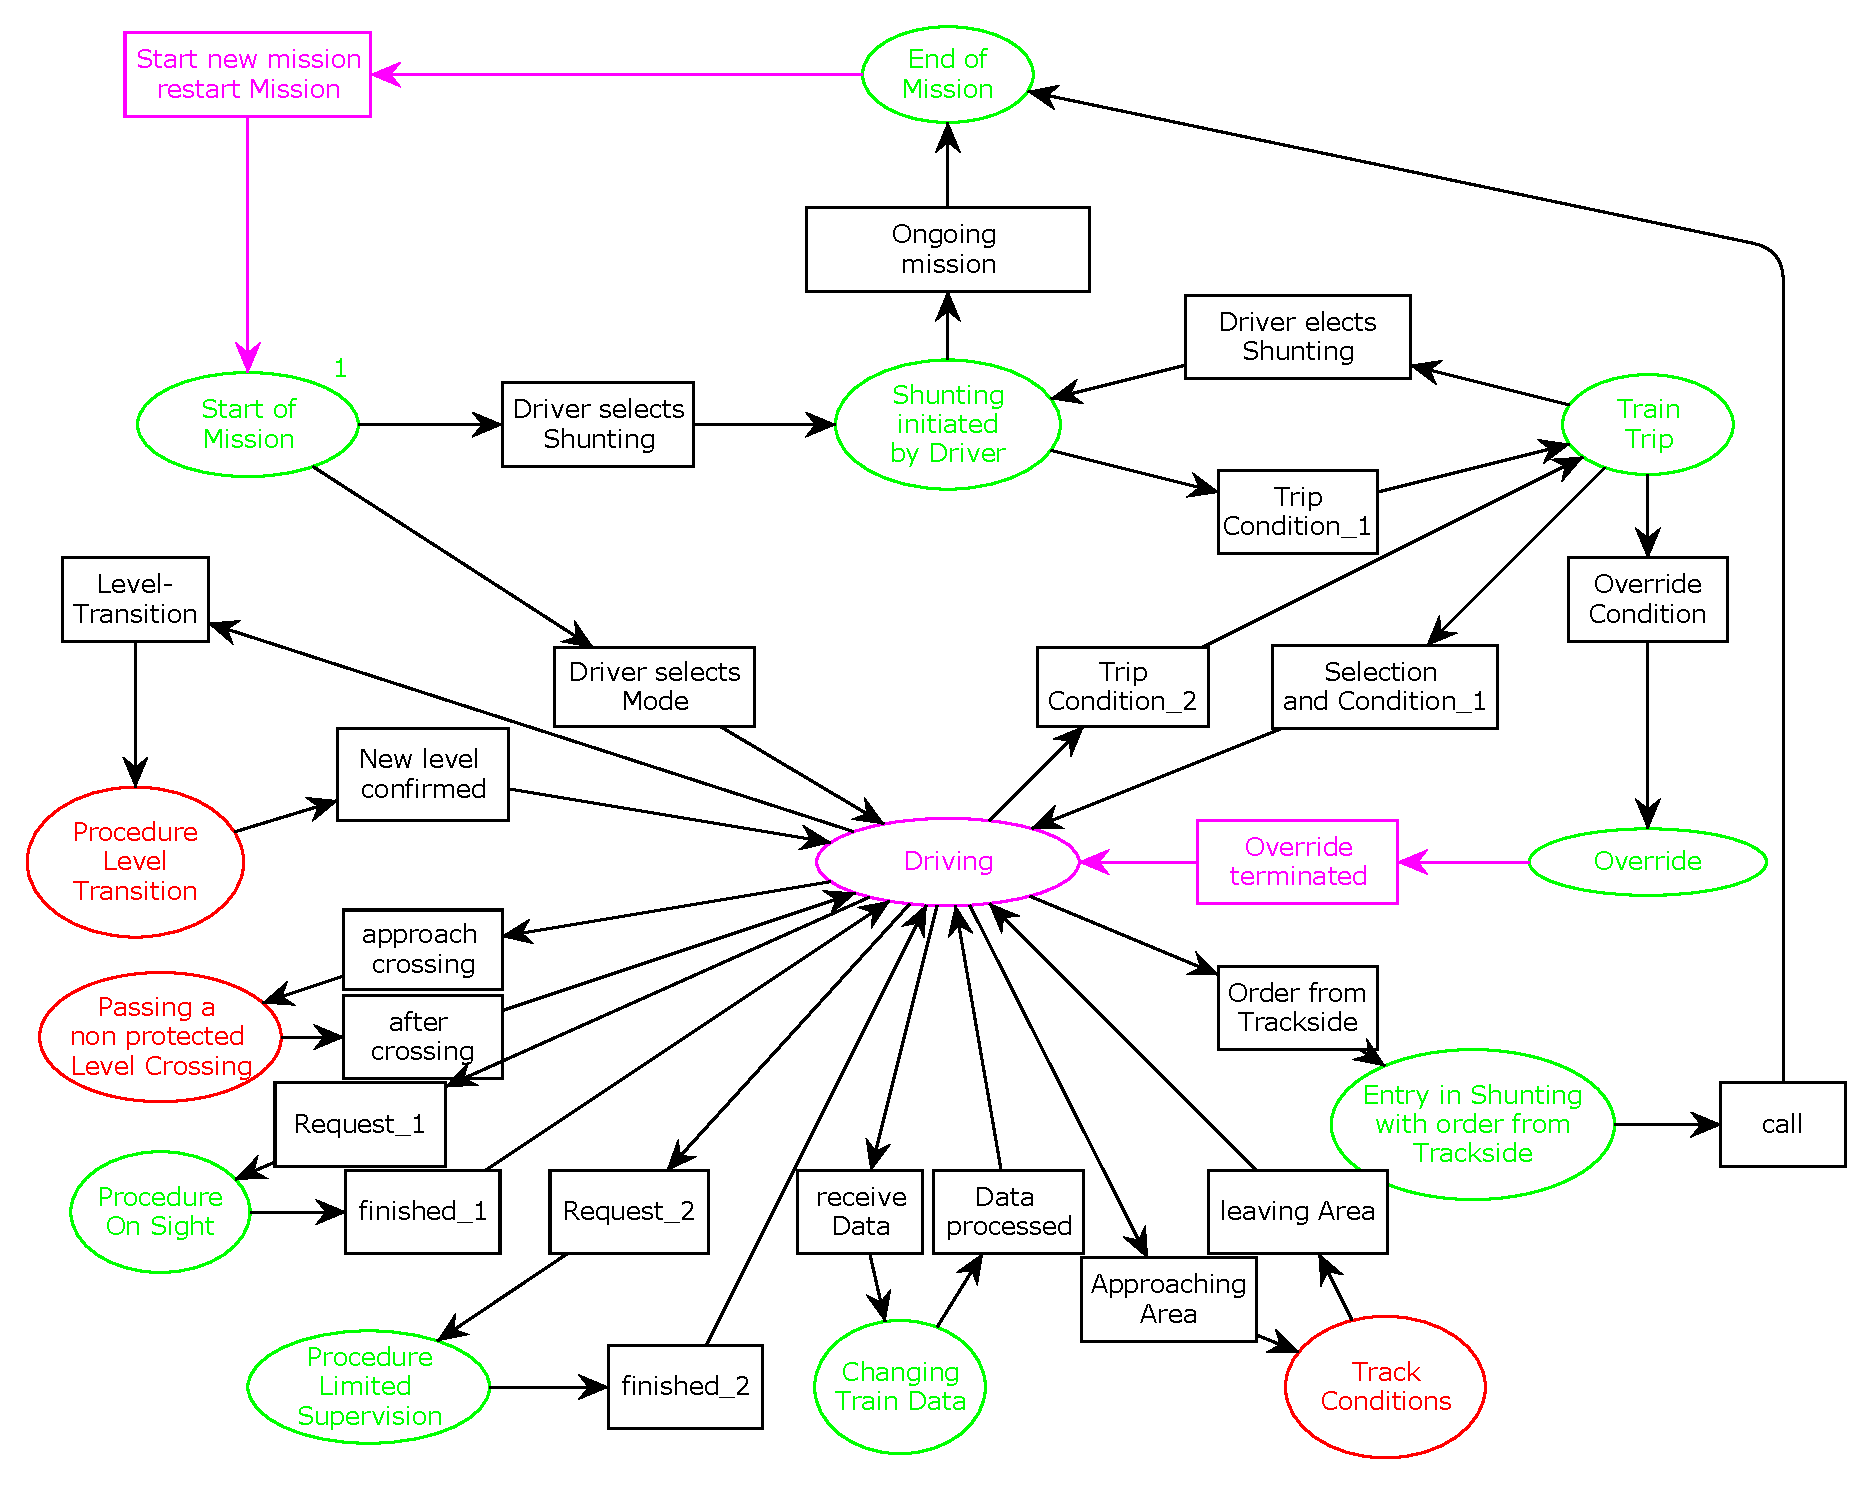
\includegraphics[width=1.0\textwidth]{Aufrufbaum.eps}
  \caption{CPN modeling the interplay of the procedures.}
  \label{fig:Bild1}
\end{figure}

In Fig.~\ref{fig:Bild1}, a procedure is modeled as a \remark{place}{Better use a substitution transition.} which is depicted as an ellipse. The name of the procedure is depicted inside the place. A transition from one procedure to another one is modeled as a transition, which is depicted as an rectangle. Again, the description of the transition is depicted inside the rectangle. In addition to the procedures there is one more place, named \textit{Driving}, which is used to model an intermediate state from which other procedures can be called.

ToDo: What do we see in Fig.~\ref{fig:Bild1}?

\subsection{Data Used in the Procedures}

In this section, we formalize the relevant data types for Chapter~5. 

The OBU can be in 17 possible modes, see Chapter~4.3.2.1. This can be defined as a set $\mathit{Mode}$ with $\mathit{Mode} = \{\mathit{FS, LS, OS, SR, SH, UN, PS, SL, SB, TR, PT, SF, IS, NP, NL, SN, RV}\}$.

There are five possible ETCS levels, i.e., $\mathit{ETCS\_Level} = \{0, 1, 2, 3, \mathit{NTC}\}$.

To communicate with its environment, the OBU sends messages to the trackside and receives messages from trackside. A message is of a particular type whereby the type is identified by a number and a description, i.e., a String. Each message type is a complex data type. We abstract from the concrete data type and define the type $\mathit{MessageType}$. We define messages from and to the driver as well as messages from and to the RBC: $\mathit{MessageToDriver} = \mathit{MessageType}$, $\mathit{MessageFromDriver} = \mathit{MessageType}$, $\mathit{MessageToRBC} = \mathit{MessageType}$, and $\mathit{MessageFromRBC} = \mathit{MessageType}$.

The Train Position Data defines the position of the train front in relation to a balise group. Train Data contains information about the train, such as its length and braking parameters. The Train Running Number and the Driver ID are identifiers. The RBC ID is the phone number of a RBC. The Virtual Balise Cover (VBC) contains a list of balises and a period of validity. However, for most data stored in the OBU we only need the status rather than the concrete value. We formalize the status using the data type $\mathit{DATASTATE} = \{\mathit{valid}, \mathit{invalid}, \mathit{unknown}\}$. To this end, the specification defines the following types, each of them of type $\mathit{DATASTATE}$:

$\mathit{DriverID}$, $\mathit{Level}$, $\mathit{RBC\_ID}$, $\mathit{TrainData}$, $\mathit{TrainRunningNumber}$, $\mathit{TrainPosition}$, $\mathit{VirtualBaliseCover}$, $\mathit{RadioNetworkID}$.

%$\mathit{TrainPositionData} = ( \mathit{ETFEP} , \mathit{CI} , \mathit{DI} , \mathit{L} )$, where \mathit{ETFEP} is the estimated train front end position with $\mathit{ETPEP} = | \mathit{FrontPosition} - \mathit{BalisePosition} |$. 
%\mathit{CI} is the confidence interval, \mathit{DI} is direction information and $L$ is a list of alternative balises.
%The Train Running Number is a non-empty concatenation of digits and possibly letters or in EBNF:
%\begin{verbatim}
%TrainRunningNumber ::= Identifier
%Identifier ::= Digit { Digit | Letter} | Letter { Digit | Letter}
%\end{verbatim}

 

  

\subsubsection{Start of Mission}

We list the relevant data types for the procedure. 

While executing the procedure, the OBU communicates with the driver and the RBC. In addition to the mode and the ETCS level, the status of the following data is relevant: $\mathit{DriverID}$, $\mathit{ETCS\_Level}$, $\mathit{RBC\_ID}$, $\mathit{TrainData}$, $\mathit{TrainRunningNumber}$, $\mathit{TrainPosition}$, $\mathit{VirtualBaliseCover}$, and $\mathit{RadioNetworkID}$.

Furthermore, the procedure checks whether the desk of the driver is open or closed, accesses and modifies the set of active RBC sessions as well as the mobile terminals that are registered to the radio network.

To start a mission, the OBU has to be in mode $\mathit{SB}$.

\subsubsection{End of Mission}

We list the relevant data types for the procedure. 

While executing the procedure, the OBU communicates with the RBC. In addition to the ETCS level, the status of the following data is relevant: $\mathit{ETCS\_Level}$, $\mathit{TrainData}$, $\mathit{RIU\_Session\_Active}$ and $\mathit{RBC\_Session\_Active}$

\subsubsection{Shunting Initiated by Driver}

While executing the procedure, the OBU communicates with the RBC. In addition to the ETCS level and the mode, the status of the following data is relevant: $\mathit{STM trip procedure}$, $\mathit{TrainPositionData}$.

\subsubsection{Entry in Shunting with Order from Trackside}

$\mathit{Mode}_{\mathit{SOT}} = \{FS, LS, OS, SR, SB, PT, UN, SN\} \subset\mathit{Mode}$

\subsubsection{Override}

We list the relevant data types for the procedure. 

While executing the procedure, the OBU communicates with the driver. In addition to the mode and the ETCS level, the status of the following data is relevant: $\mathit{TrainData}$

The mode is in $\mathit{Mode}_{\mathit{Override}} = \{FS, LS, OS, SR, SH, SB, PT, UN, SN\} \subset\mathit{Mode}$

\subsubsection{On-Sight}

While executing the procedure, the OBU communicates with the driver.

$\mathit{Mode}_{\mathit{OS}} = \{FS, LS, OS, SR, SB, PT, UN, SN\} \subset\mathit{Mode}$

\subsubsection{Level Transitions}

\subsubsection{Train Trip}

While executing the procedure, the OBU communicates with the driver and the RBC. In addition to the mode and the ETCS level, the status of the following data is relevant: $\mathit{TrainData}$

\subsubsection{Change of Train Orientation}

\subsubsection{Train Reversing}

\subsubsection{Joining / Splitting}

\subsubsection{RBC/RBC Handover}

\subsubsection{Procedure Passing a Non-protected Level Crossing}

\subsubsection{Changing Train Data from Sources Different from the Driver}

$\mathit{Mode}_{\mathit{CTD}} = \{FS, LS, OS, SR, SB, PT, UN, SN, SH\} \subset\mathit{Mode}$

\subsubsection{Indication of Track Conditions}

\subsubsection{Limited Supervision}

While executing the procedure, the OBU communicates with the driver.

$\mathit{Mode}_{\mathit{LS}} = \{FS, LS, OS, SR, SB, PT, UN, SN\} \subset\mathit{Mode}$


\section{CPN Models}\label{s:CPNmodels}

\subsection{Design decisions}

We do not model unidirectional messages, as this would result in a possible unbounded model or would cause modeling overhead to delete those messages immediately.

\subsection{Data abstraction}

Instead of considering all possible active RBC session, we only consider whether there exists at least one active RBC session or not. Thus, we model this as a Boolean $\mathit{ActiveRBCSession} = \{\mathit{true}, \mathit{false}\}$. Similar we abstract from the information of the mobile terminal being registered to a radio network and model it as a Boolean $\mathit{MobileTerminalRegisteredToRadioNetwork} = \{\mathit{true}, \mathit{false}\}$.

We further abstract from concrete messages---that is, the content of a message. To identify which message type has been sent by the OBU to the driver or the RBC, we abstract those messages to a String, i.e., $\mathit{MessageToDriver} = \mathit{MessageToRBC} = \mathit{String}$. A message from the RBC is abstracted to an undistinguishable black token, i.e., $\mathit{MessageFromRBC} = \mathit{UNIT}$. From a message sent by the driver, we are only interested whether or not the driver conforms a request; thus, the abstracted data type is of type Boolean, i.e., $\mathit{MessageFromDriver} = \mathit{Bool}$. Decisions based on on received data are modeled using a nondeterministic choice. As result, our model is a safe over-approximation of the concrete system.

\subsection{Property preservation}

If there exists a path in the concrete system, then there also exists a path in the model (but not necessarily the other way around).

\subsection{Start of Mission}
\subsubsection{Assumptions}
\subsubsection{Interface}

Figure~\ref{fig:SoM-toplevel} shows the top level model of Start of Mission and its environment. 
\begin{figure}[htb] 
  \centering
  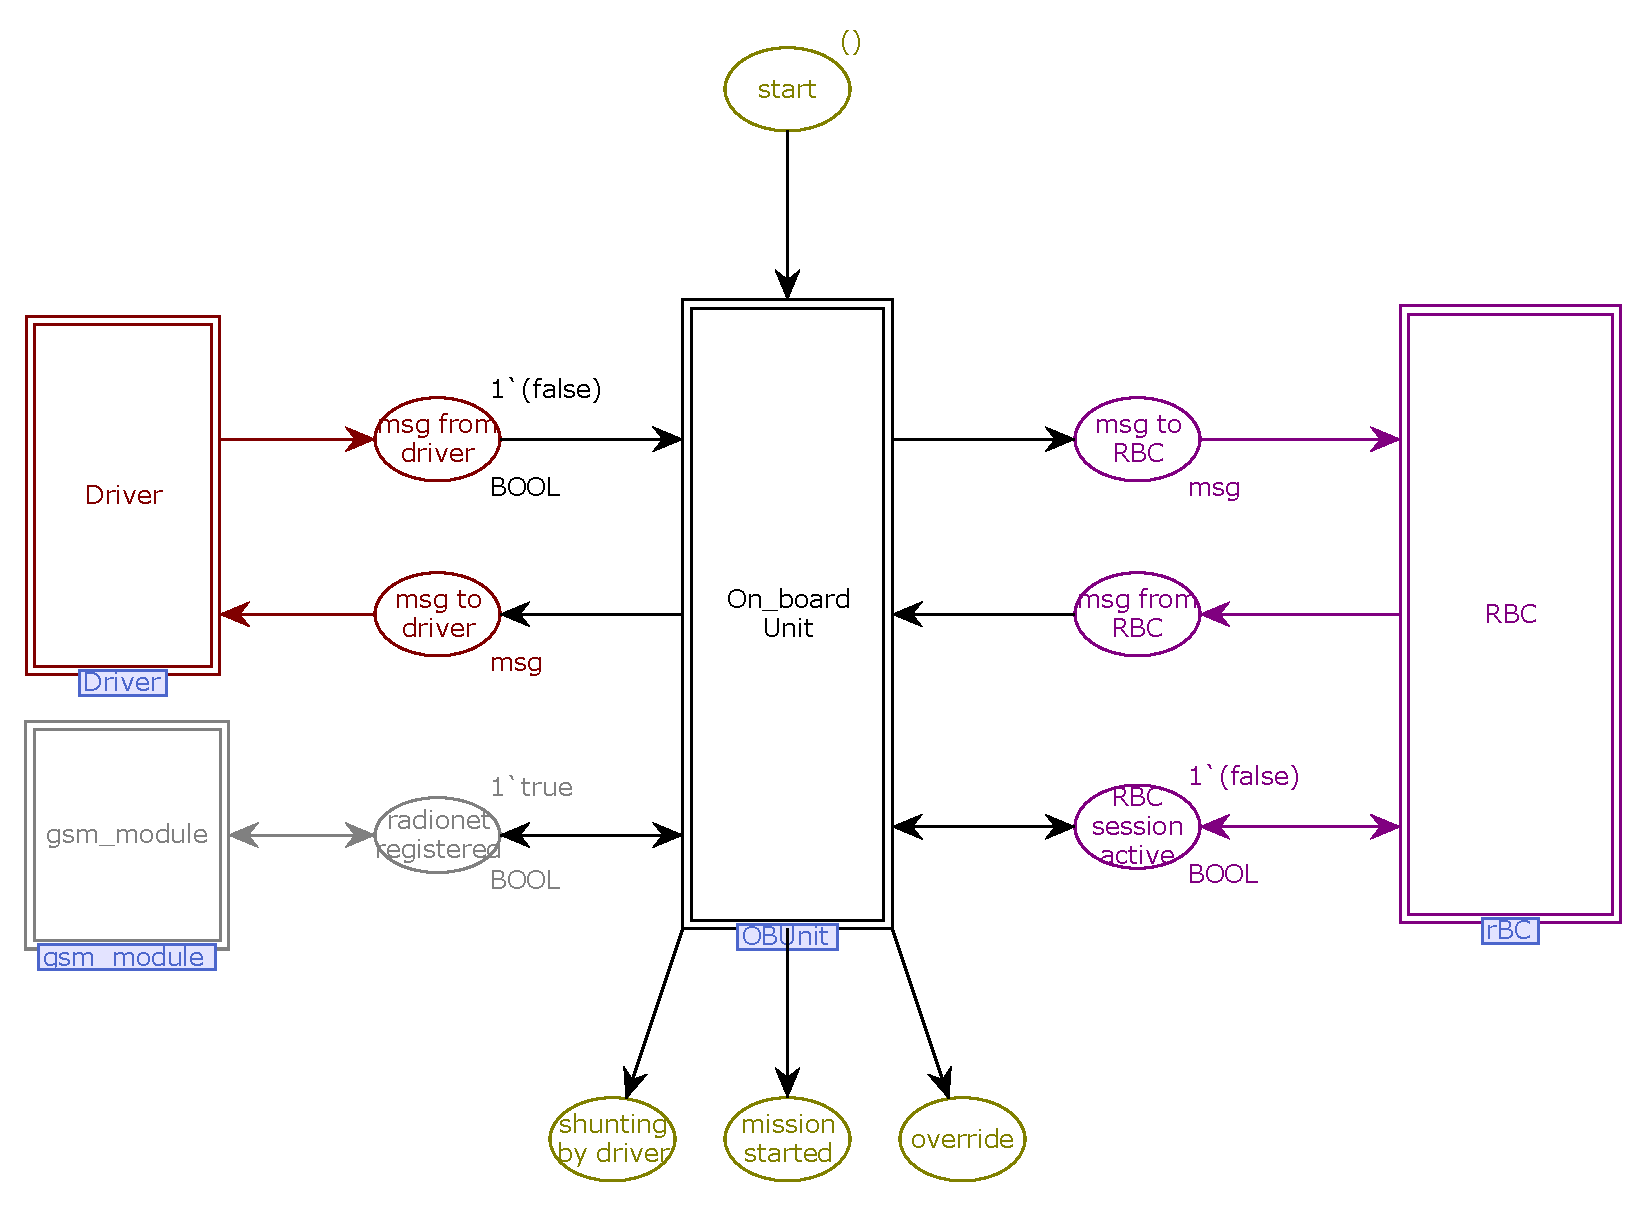
\includegraphics[scale=0.5]{SoM-toplevel.eps}
  \caption{Top level model of Start of Mission and its environment}
  \label{fig:SoM-toplevel}
\end{figure}

We model an interface to the driver and to the RBC. In addition, $\mathit{MobileTerminalRegisteredToRadioNetwork}$ serves as an interface to the GSM module. The following places model the interface:
\begin{description}
	\item[place ``msg to driver''] $\mathit{MessageToDriver}$
	%
	\item[place ``msg from driver''] $\mathit{MessageFromDriver}$
	%
	\item[place ``msg to RBC''] $\mathit{MessageToRBC}$
	%
	\item[place ``msg from RBC''] $\mathit{MessageFromRBC}$
	%
	\item[place ``RBC session active''] $\mathit{ActiveRBCSession}$
	%
	\item[place ``radionet registered''] $\mathit{MobileTerminalRegisteredToRadioNetwork}$; interface to GSM module
\end{description}

The interface to other components (i.e., Petri nets modeling procedures other than Start of Mission) consists of four places, one input and three output places:
\begin{description}
	\item[place ``start''] input place of the component
	%
	\item[place ``shunting by driver''] output place to invoke procedure Shunting initiated by driver
	%
	\item[place ``mission started''] output place signaling that the mission has started
	%
	\item[place ``override''] output place to invoke procedure Override
\end{description}

\subsubsection{Data used}

The following data is modeled using a data place:
\begin{description}
	\item[place ``virtual balise cover''] $\mathit{VirtualBaliseCover}$
	%
	\item[place ``driver\_id''] $\mathit{DriverID}$
	%
	\item[place ``mode''] $\mathit{Mode}$
	%
	\item[place ``train\_rno''] $\mathit{TrainRunningNumber}$
	%
	\item[place ``ETCS State''] $\mathit{Level}$
	%
	\item[place ``train position data''] $\mathit{trainPositionData}$
	%
	\item[place ``ETCS level''] $\mathit{ETCS\_Level}$
	%
	\item[place ``rbc\_id''] $\mathit{RBC\_ID}$
	%
	\item[place ``train data''] $\mathit{TrainData}$
	%
	\item[place ``Radio Network ID''] $\mathit{RadioNetworkID}$
	%
	\item[place ``desk(s) open''] $\mathit{Boolean}$, models whether the desk is open
	%
	\item[place ``RBC session active''] $\mathit{ActiveRBCSession}$
	%
	\item[place ``radionet registered''] $\mathit{MobileTerminalRegisteredToRadioNetwork}$
\end{description}

Figure~\ref{fig:SoM-level1} shows the first level of the model Start of Mission. The places colored green are the data places.
\begin{figure}[htb] 
  \centering
  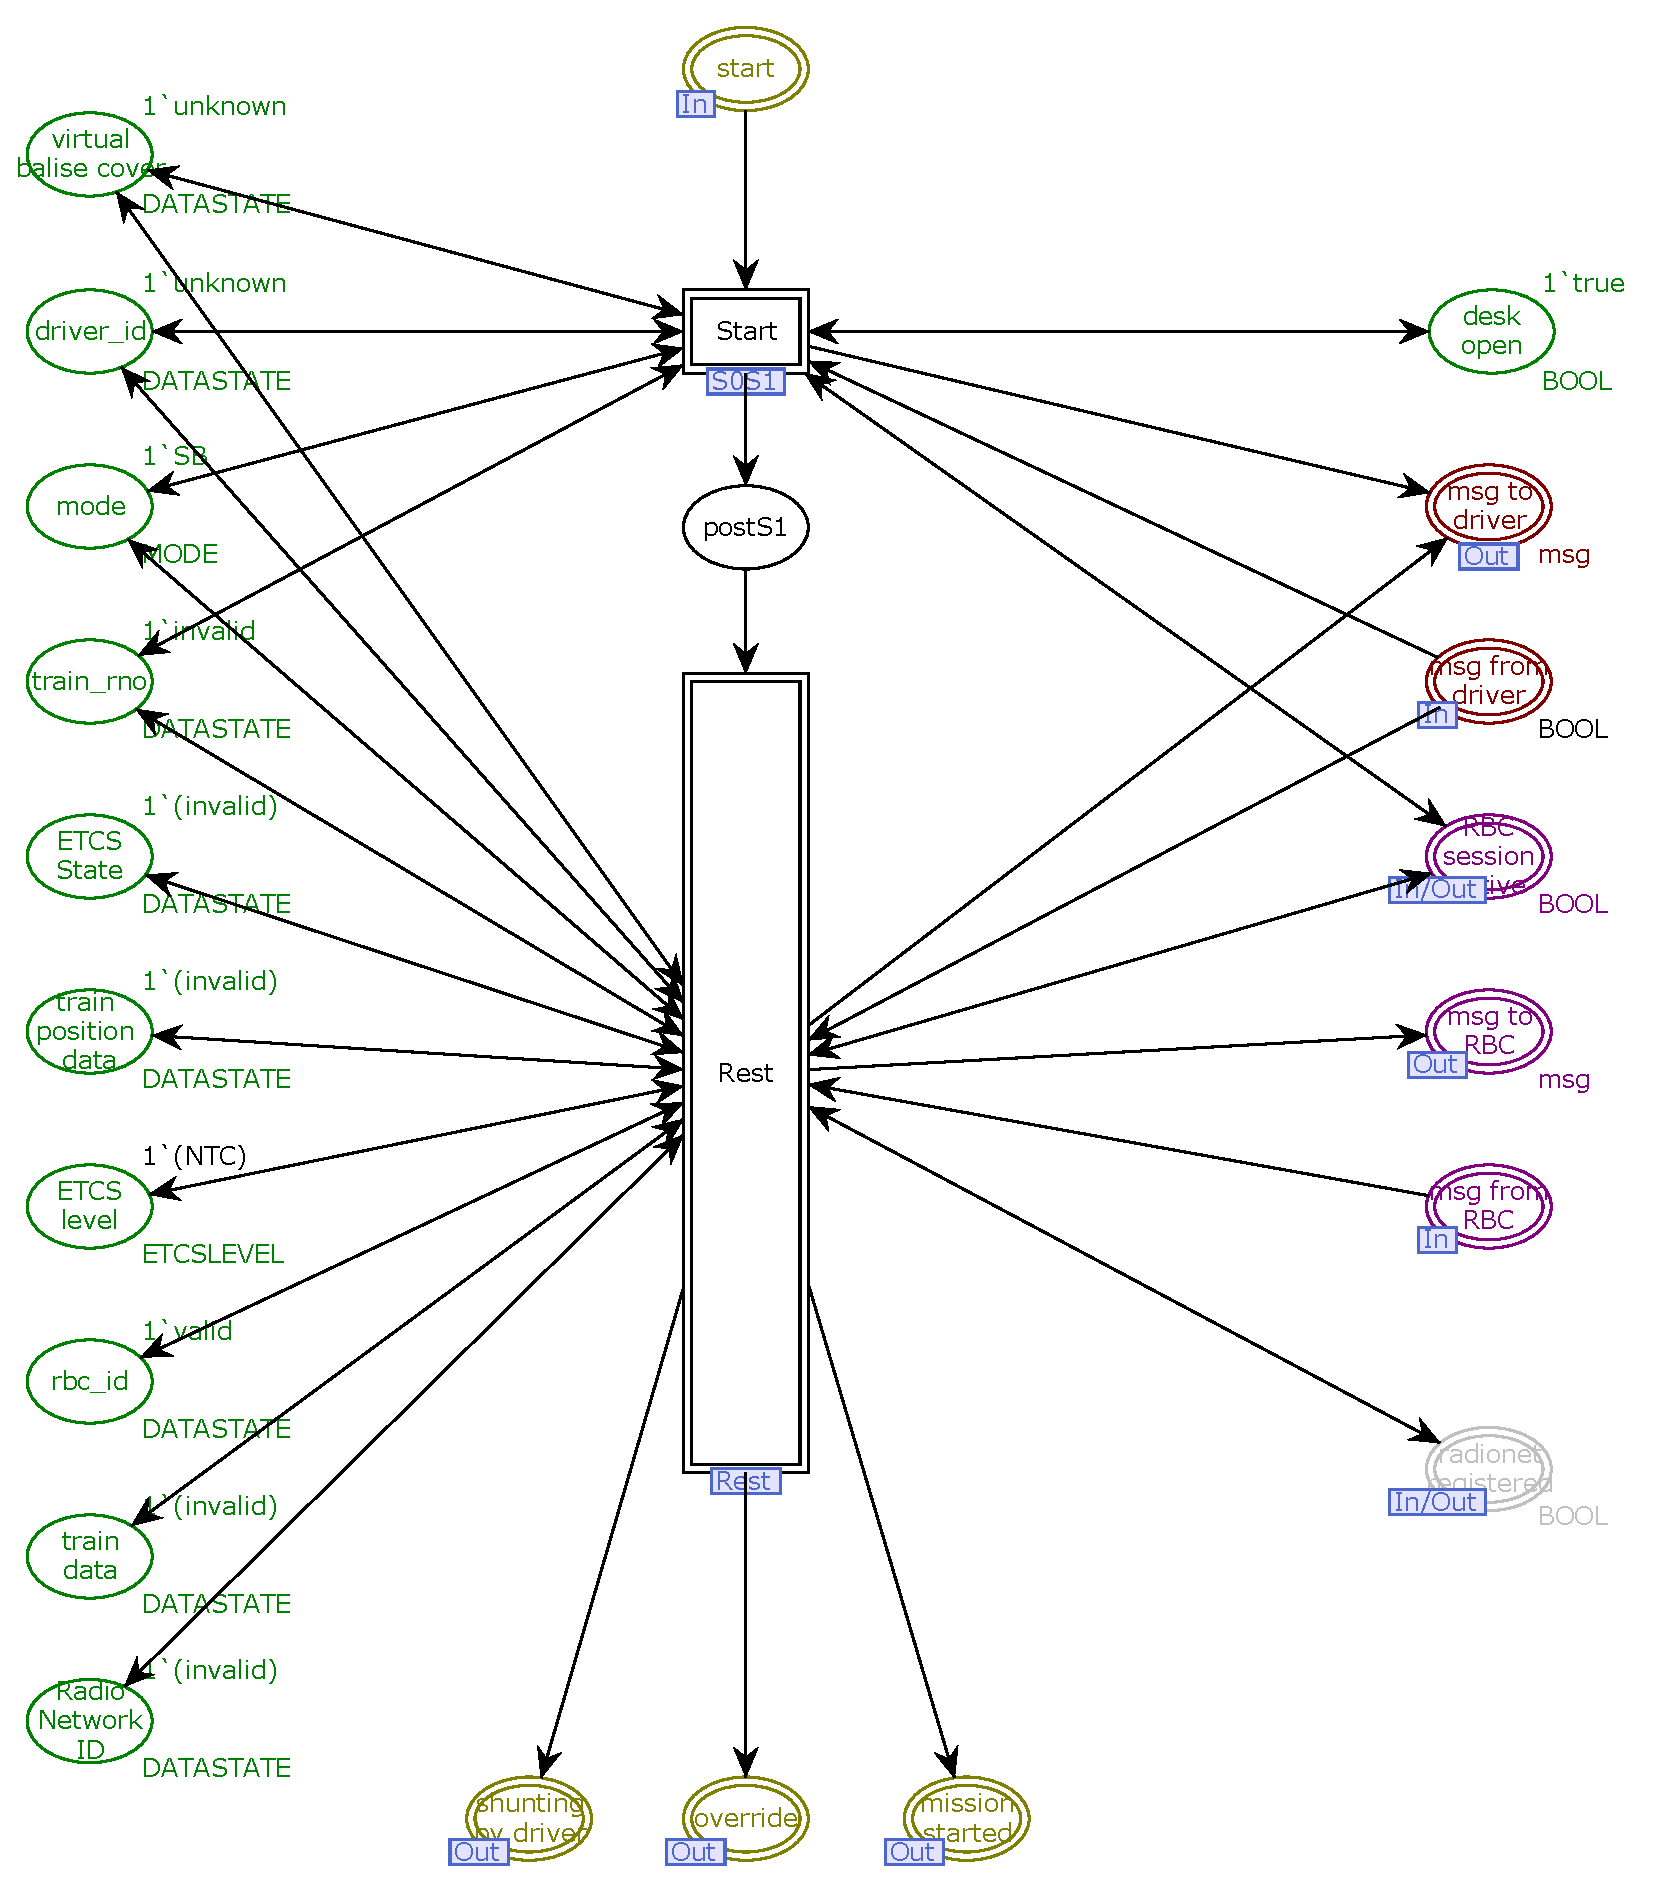
\includegraphics[scale=0.5]{SoM-level1.eps}
  \caption{First level model of Start of Mission---interface place are colored green.}
  \label{fig:SoM-level1}
\end{figure}

\subsubsection{Initial marking}

The current mode is $\mathit{SB}$.

\subsubsection{State space analysis}
First of all, the net is bounded and there are no deadlocks, except the desired exit-states.


\subsection{End of Mission}

\begin{figure}[htb] 
  \centering
  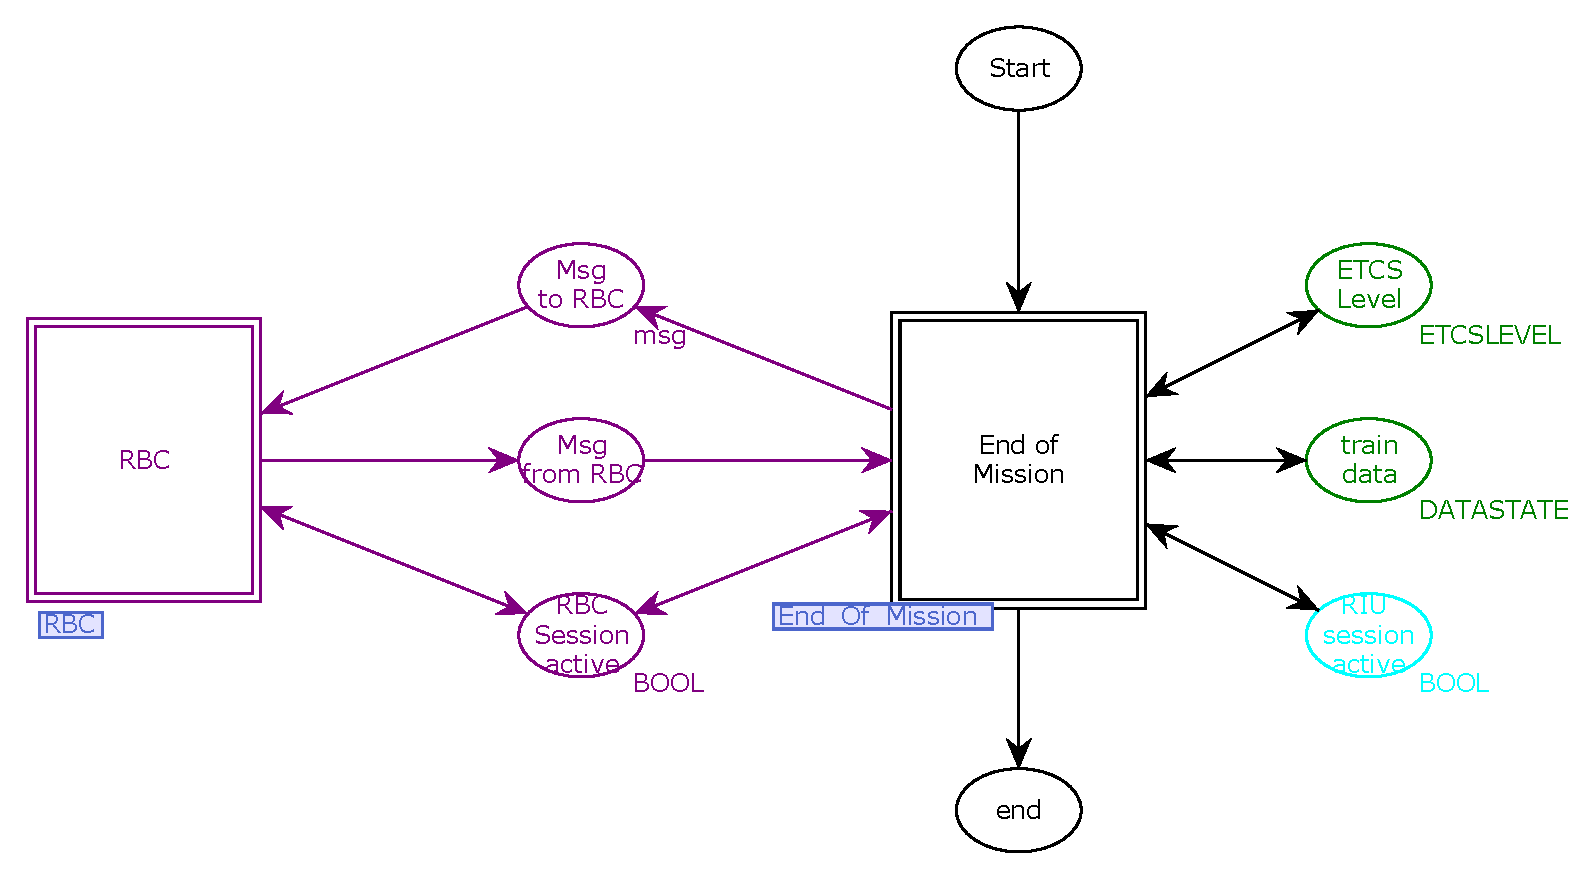
\includegraphics[scale=0.5]{EoM-toplevel.eps}
  \caption{Top level model of End of Mission and its environment}
  \label{fig:EoM-toplevel}
\end{figure}



\subsubsection{State Space Analysis}
In order to analyze the subnet in all possible scenarios, we randomly choose the initial marking.

If we assume, that a RBC-session can only be active if the ETCS-Level is 2 or 3, then the net is deadlock free. The exception of this deadlock freedom is the desired "end" state.
The net doesn't contain any dead transitions. (if we assume, that any initial marking is possible when entering the procedure.)

\subsection{Shunting Initiated by Driver}

It is not stored yet whether there is an ongoing mission.

\begin{figure}[htb] 
  \centering
  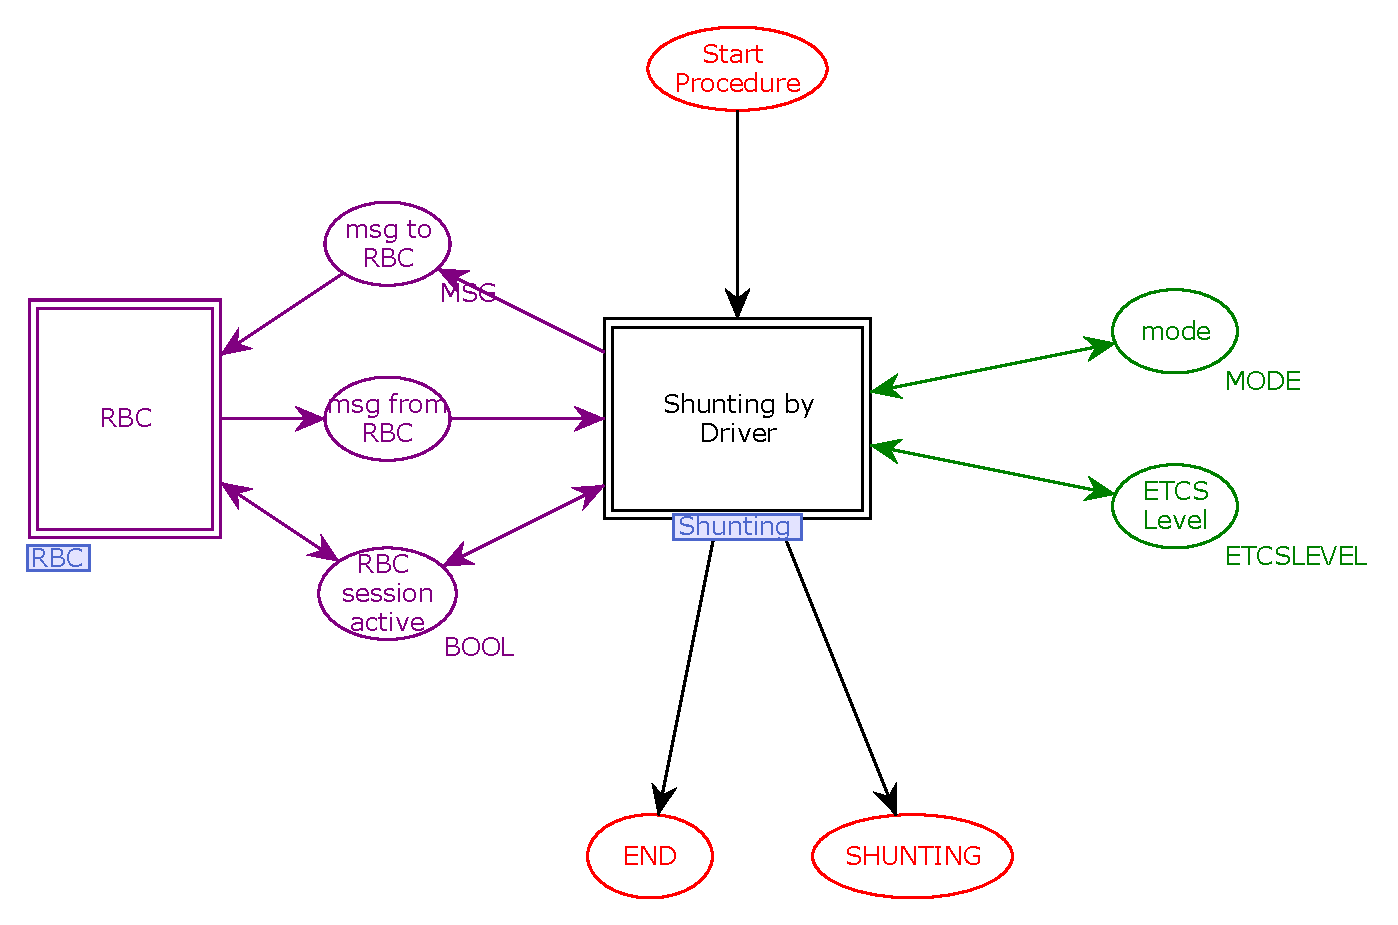
\includegraphics[scale=0.5]{ShuntingDriver-toplevel.eps}
  \caption{Top level model of Shunting Initiated by Driver and its environment}
  \label{fig:SD-toplevel}
\end{figure}

\subsection{Entry in Shunting with Order from Trackside}
\begin{figure}[htb] 
  \centering
  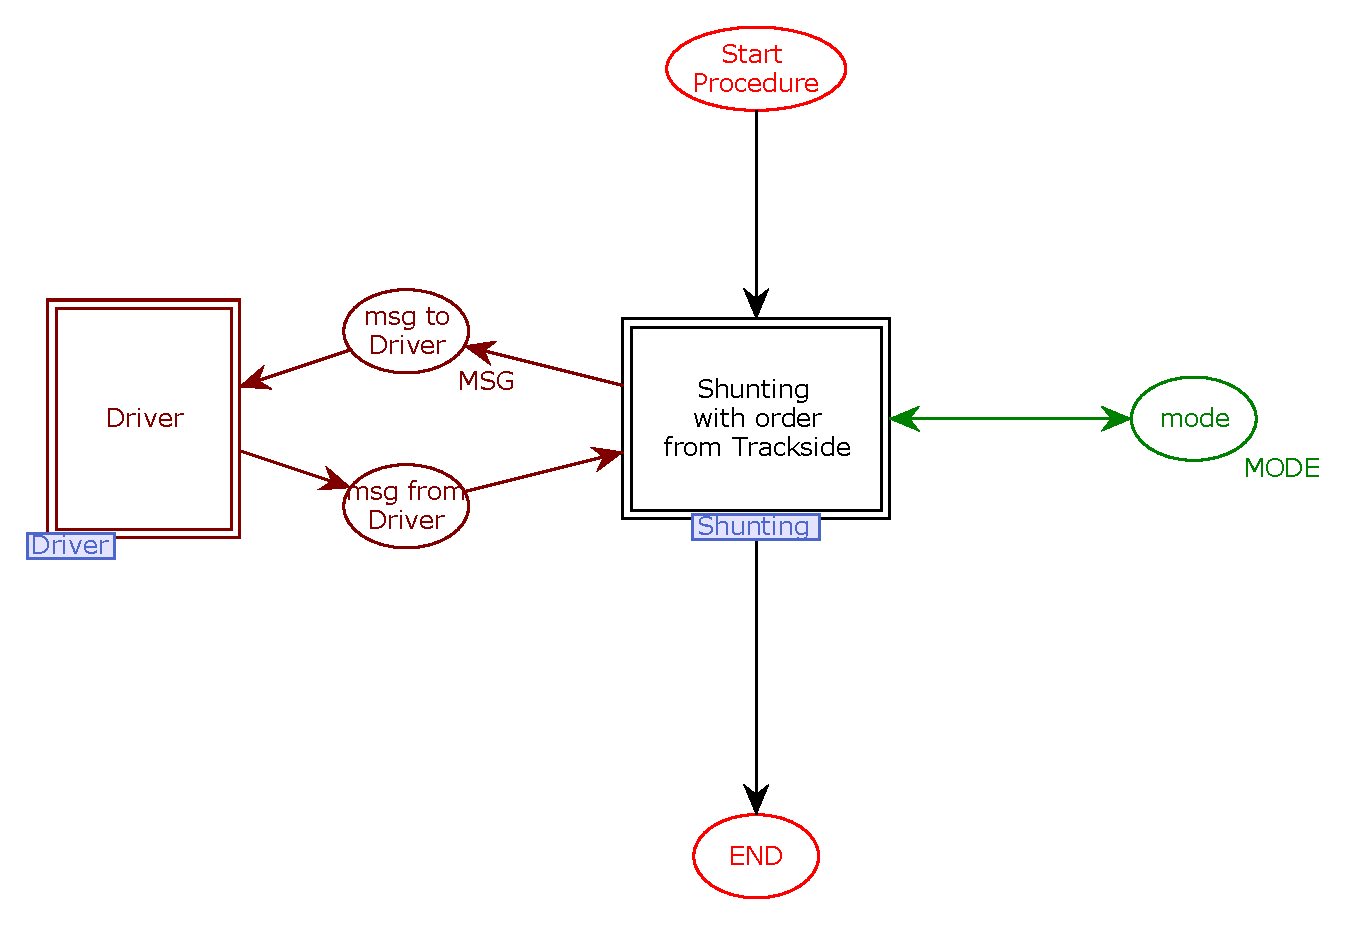
\includegraphics[scale=0.5]{ShuntingTrackside-toplevel.eps}
  \caption{Top level model of Shunting with Order from Trackside and its environment}
  \label{fig:ST-toplevel}
\end{figure}

\subsection{Override}

\begin{figure}[htb] 
  \centering
  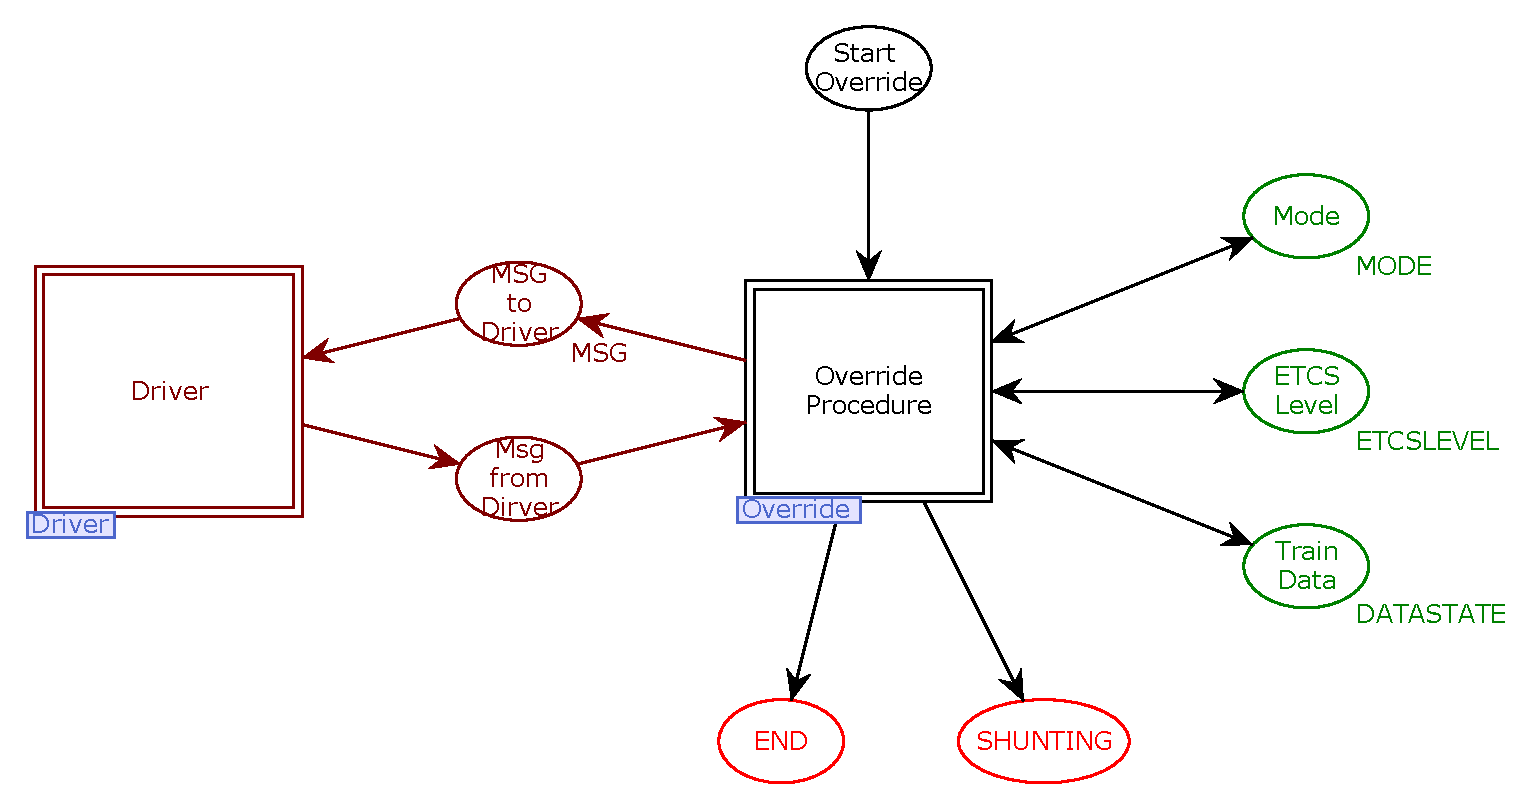
\includegraphics[scale=0.5]{Override-toplevel.eps}
  \caption{Top level model of Override and its environment}
  \label{fig:Override-toplevel}
\end{figure}

If we decided to model movement authorities, then, in level 2 and 3, there would be communication with the RBC where messages can be lost.

\subsubsection{initial marking}
The Train Data is valid.
The mode is Full Supervision, Limited Supervision, On Sight, Staff Responsible, Shunting, Unfitted, Post Trip, Stand By (in level 2/3 only) or SN.
All other variables are chosen randomly, thus ensuring that every possible scenario is covered.

\subsubsection{State space analysis}

The state space contains 212 nodes and 418 edges.
There are no deadlocks and the net is bounded.
 


\subsection{On-Sight}
\begin{figure}[htb] 
  \centering
  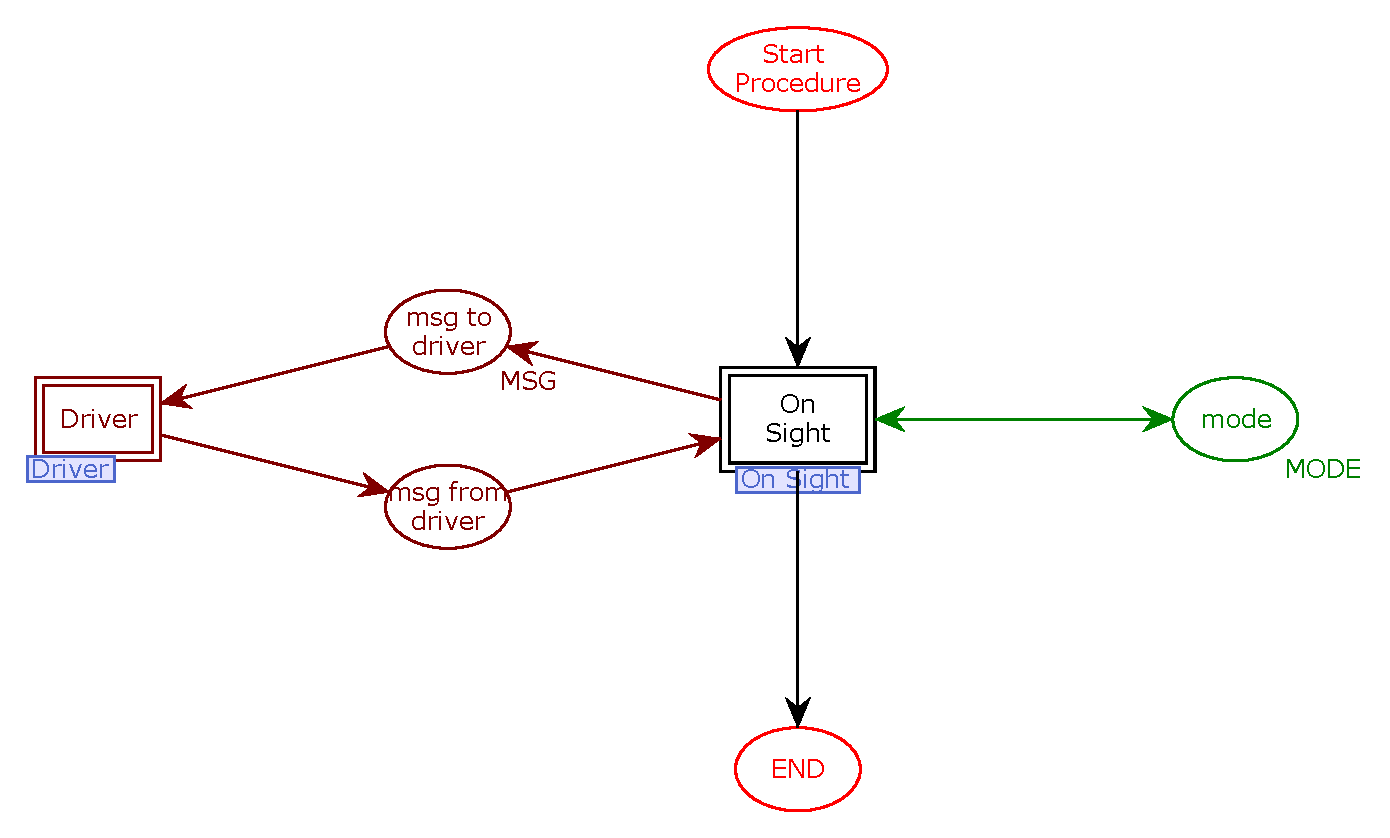
\includegraphics[scale=0.5]{OnSight-toplevel.eps}
  \caption{Top level model of On Sight and its environment}
  \label{fig:On Sight-toplevel}
\end{figure}

\subsection{Level Transitions}

\subsection{Train Trip}

\begin{figure}[htb] 
  \centering
  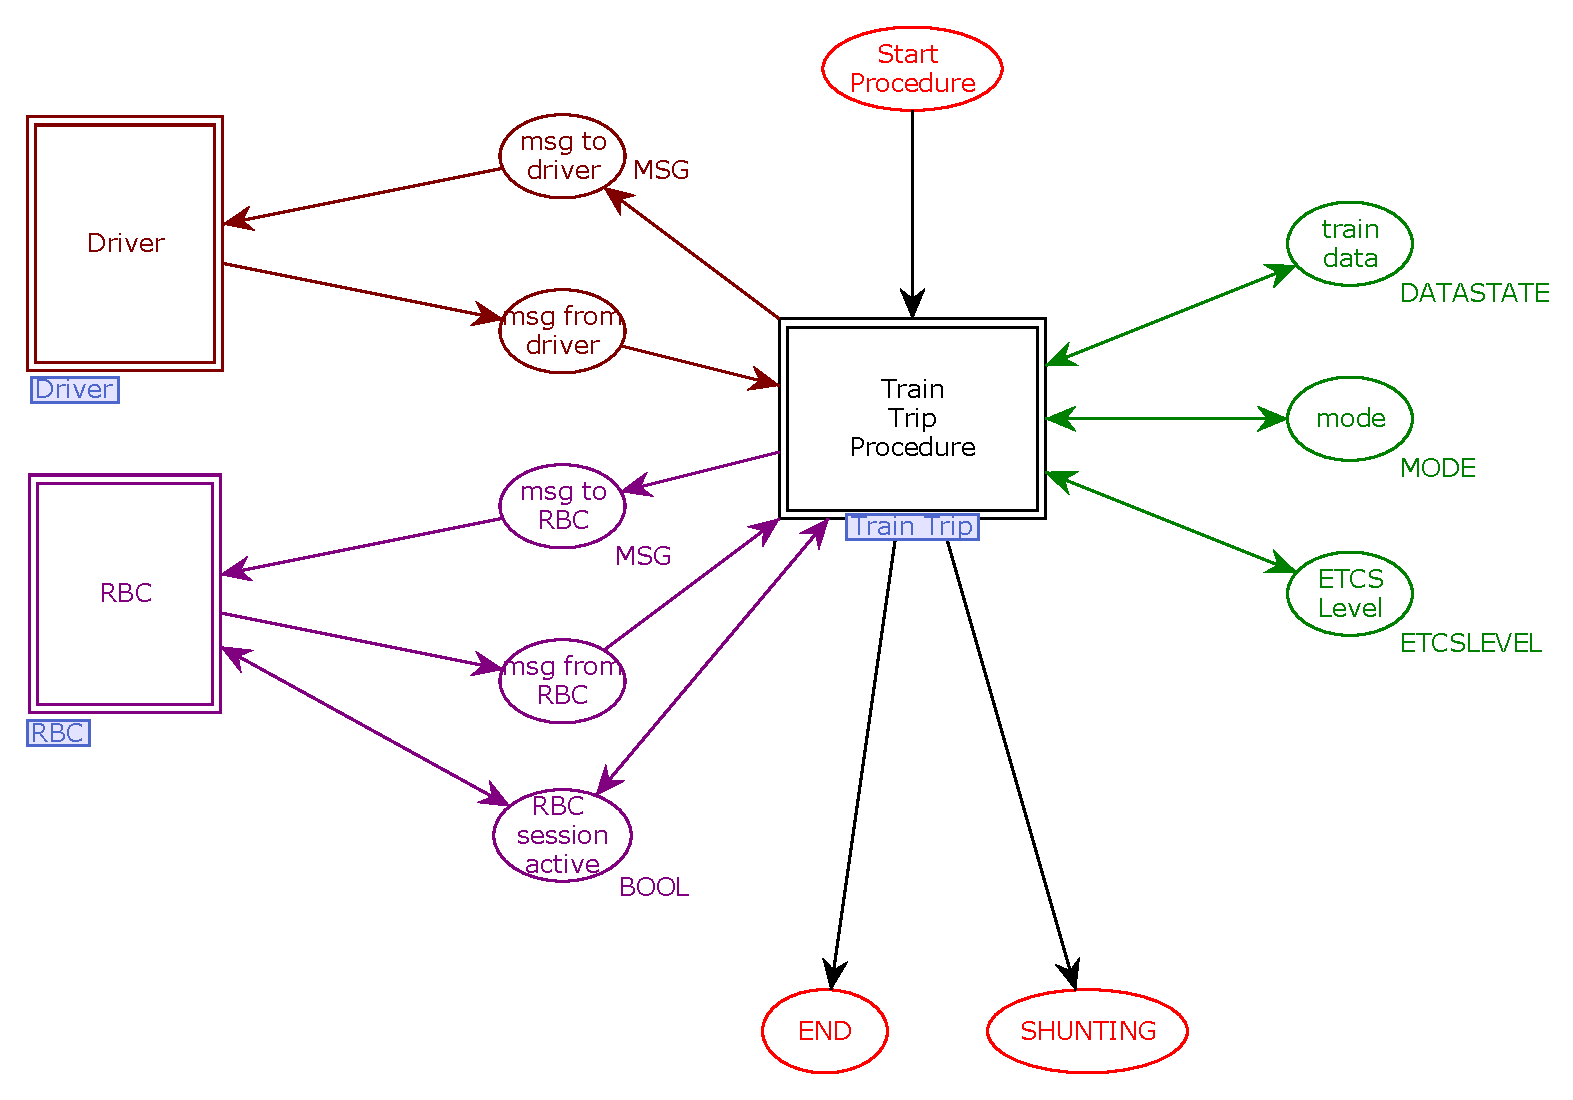
\includegraphics[scale=0.5]{Train_Trip-toplevel.eps}
  \caption{Top level model of Train Trip and its environment}
  \label{fig:Trip-toplevel}
\end{figure}

\subsection{Change of Train Orientation}

\subsection{Train Reversing}

\subsection{Joining / Splitting}

\subsection{RBC/RBC Handover}

\subsection{Procedure Passing a Non-protected Level Crossing}

\subsection{Changing Train Data from Sources Different from the Driver}

\begin{figure}[htb] 
  \centering
  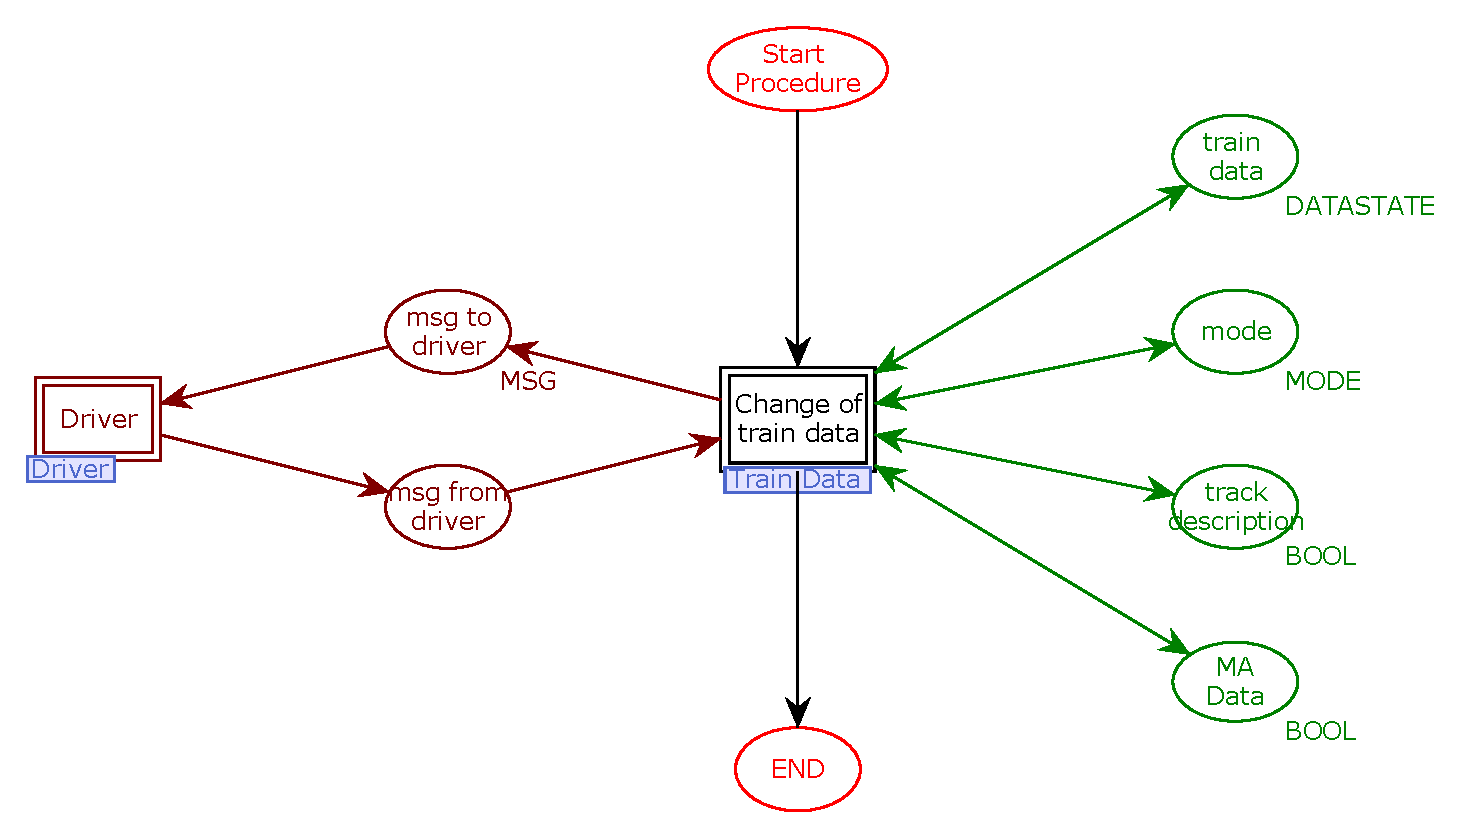
\includegraphics[scale=0.5]{CoTD-toplevel.eps}
  \caption{Top level model of Change of Train Data and its environment}
  \label{fig:Change of Train Data-toplevel}
\end{figure}

\subsection{Indication of Track Conditions}

\subsection{Limited Supervision}

\begin{figure}[htb] 
  \centering
  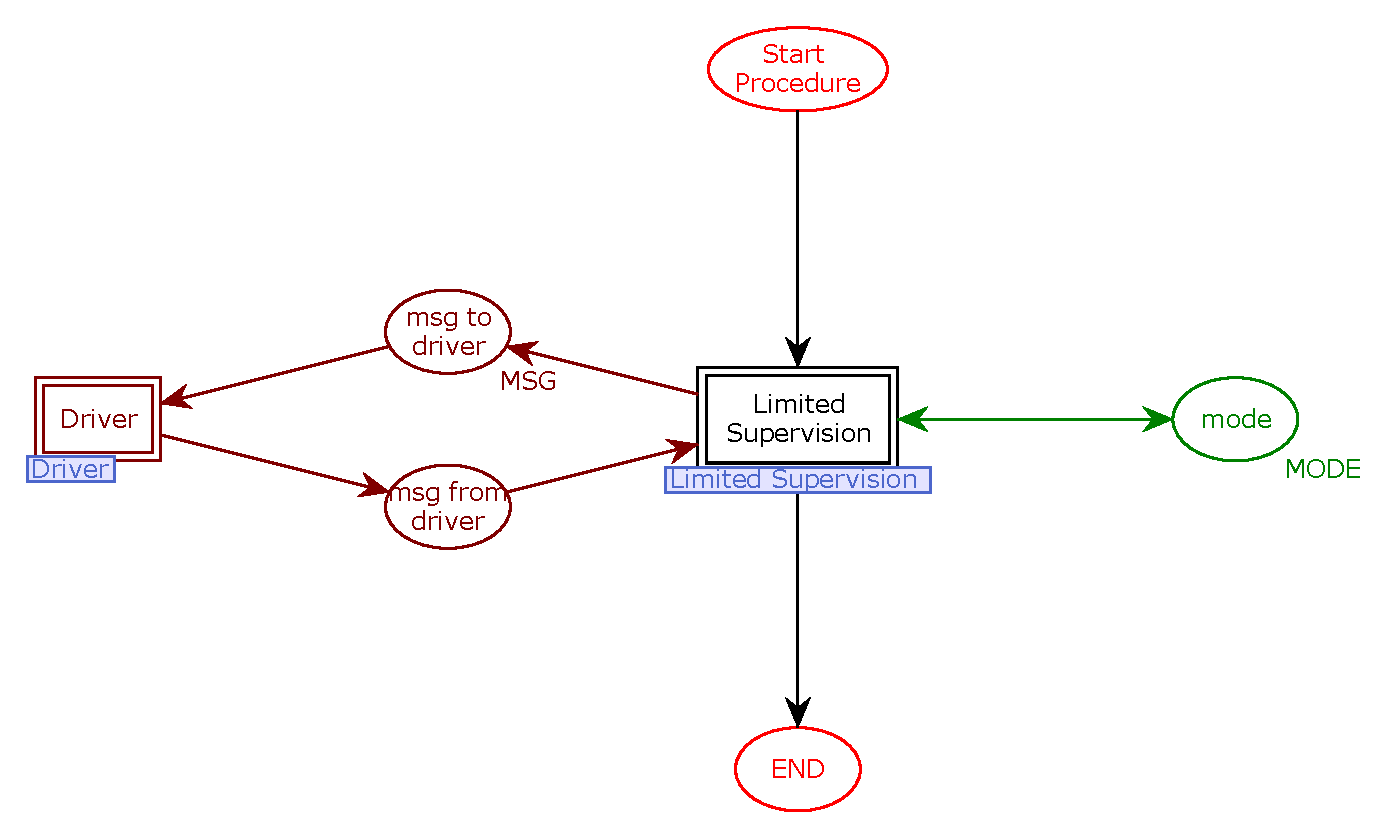
\includegraphics[scale=0.5]{LimitedSuper-toplevel.eps}
  \caption{Top level model of Limited Supervision and its environment}
  \label{fig:Limitedsup-toplevel}
\end{figure}



\section{Validation of the specification}\label{s:validation}

\subsection{Specification findings}

\subsection{Considered scenarios/properties}

\begin{comment}

\section{Overview of the CPN Approach}

\subsection{Coverage of the Specification}
The current coverage of the specification can be derived from the Call Graph.
The green-colored procedures have been already modeled, whereas the red ones are yet to be included in the model.



\subsection{Call Graph}
\begin{figure}[htbp] 
  \centering
     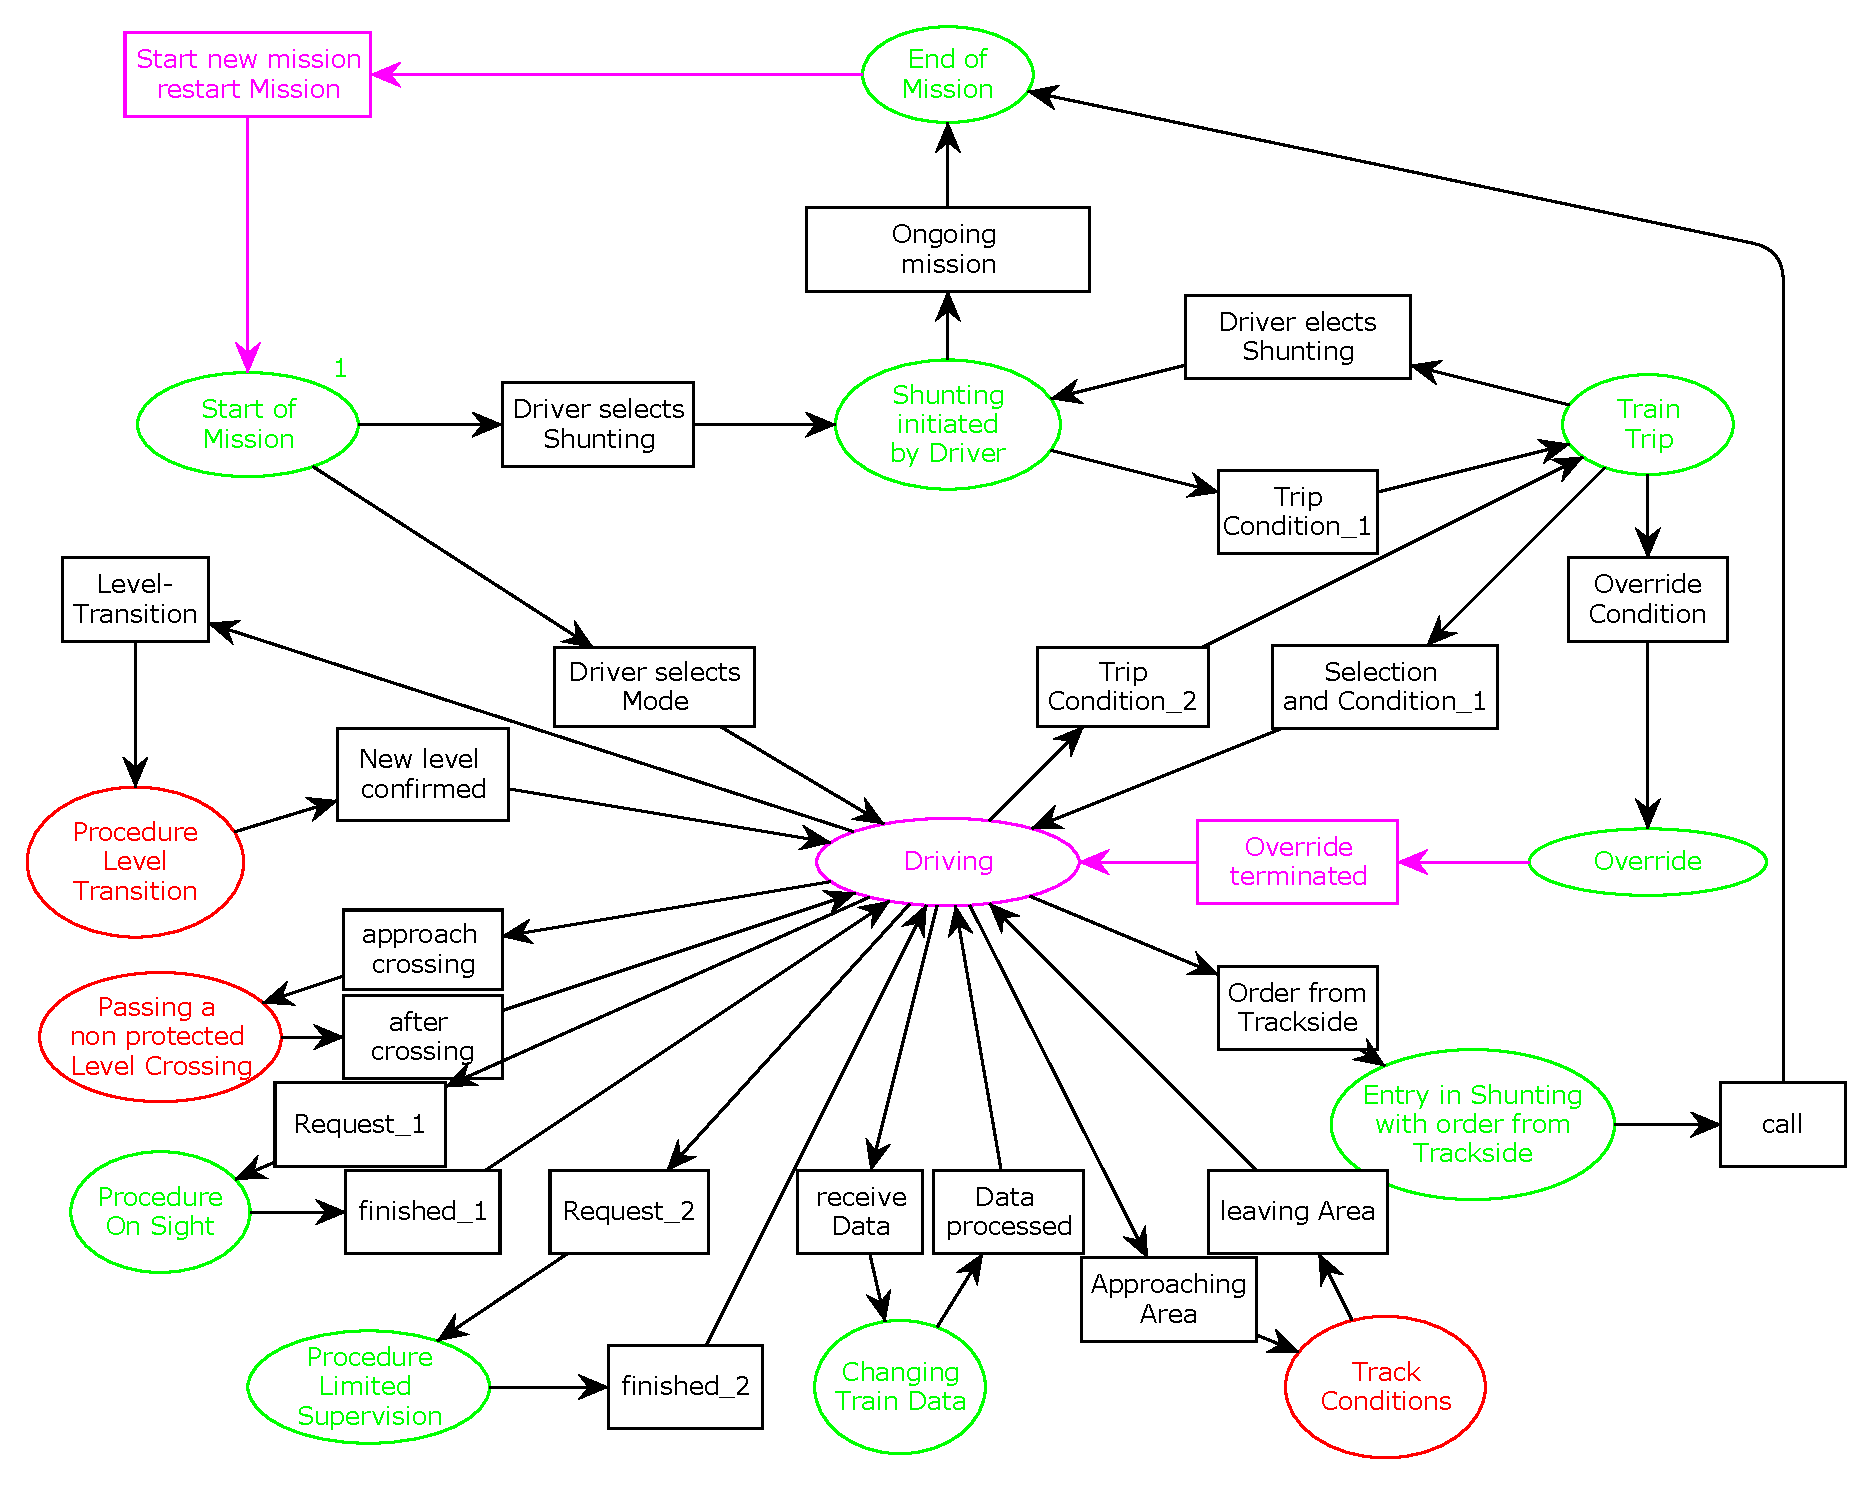
\includegraphics[width=1.0\textwidth]{Aufrufbaum.eps}
  \caption{Call Graph of the procedures}
  \label{fig:Bild1}
\end{figure}

\subsection{Occurrence of time in the specification}
\begin{enumerate}
\item In 5.5.4, there is a "fixed waiting time", after which a message is to be sent again.
\item In 5.6.4.1.1 the same "fixed waiting time" occurs.
\item 5.7.2.4 (and 5.7.3.7 etc.) mentions a "driver acknowledgement time". (5 seconds) If the driver doesn't acknowledge a mode change during this time, the trains emergency brake will take effect.
\item 5.8.4.1.a: there is a "max. time for train trip suppression when Override function is triggered." After this time, the Override procedure shall end.
\item 
\end{enumerate}


\section{Partitioning CPNs}



\subsection{Procedure On Sight}
\begin{enumerate}
	\item Prerequisites: 
		\begin{enumerate}
			\item mode is FS, LS, OS, SR, SB, PT, UN, or SN
			\item intentionally left blank ;)
		\end{enumerate}  
		
	\item Connected instances and used data
	\begin{enumerate}
		\item Communication with the driver
		\item Access to the current mode
		\item Communication with balise groups, not modeled yet!
	\end{enumerate}		 
	\item Abstractions and characteristics of the examined model
		\begin{enumerate}
			\item we assume that the driver will acknowledge a request finally or else the procedure can`t terminate.
			\item in order to reach all states and transitions the procedure starts with three markings on the place "mode". In reality there can be only one marking on that place.
			\item To prevent the end of procedure place from being a dead state we introduced a new transition. Once the system is in the "end" place only the new transition can be fired and firing the transition will again lead into the "end" place. Thus whenever there occurs a dead state in our analysis, it is an error.
			
		\end{enumerate}
	\item results of the state space analysis
	
		\begin{enumerate}
			\item The state space contains 287 nodes and 554 arcs.
			\item there are no dead states
			\item there are no unbounded states
			\item all places and transitions can be reached
			\item there can be two messages to the driver at the same time, which might be a problem
			
			
		\end{enumerate}
\end{enumerate}

The full report, as created by the CPN-tools state-space tool can be found in the "State-Spaces" folder by the name "SS\_On\_Sight.txt".


\subsection{Procedure Limited Supervision}

This procedure is very similar to the procedure On Sight. 

\begin{enumerate}

\item Prerequisites: 
		\begin{enumerate}
			\item mode is FS, LS, OS, SR, SB, PT, UN, or SN
			\item intentionally left blank ;)
		\end{enumerate} 
	\item Connected instances and used data
		\begin{enumerate}
			\item Communication with the driver
			\item Access to the current mode
			\item Communication with balise groups, not modeled yet!
		\end{enumerate}  
	\item Abstractions and characteristics of the examined model
		\begin{enumerate}
			\item we assume that the driver will acknowledge a request finally or else the procedure can`t terminate.
			\item in order to reach all states and transitions the procedure starts with three markings on the place "mode". In reality there can be only one marking on that place.
			\item To prevent the end of procedure place from being a dead state we introduced a new transition. Once the system is in the "end" place only the new transition can be fired and firing the transition will again lead into the "end" place. Thus whenever there occurs a dead state in our analysis, it is an error.
			
		\end{enumerate}
	\item results of the state space analysis
	
		\begin{enumerate}
			\item The state space contains 227 nodes and 336 arcs.
			\item there are no dead states
			\item there are no unbounded states
			\item all places and transitions can be reached
			\item there can be two messages to the driver at the same time, which might be a problem
			
			
		\end{enumerate}
\end{enumerate}



\subsection{Procedure Shunting with order from Trackside}

This procedure is very similar to the procedure On Sight. The main exception is, that it is not possible to enter the procedure when already in shunting mode. Thus one branch is missing. 

\begin{enumerate}

\item Prerequisites: 
		\begin{enumerate}
			\item mode is FS, LS, OS, SR, SB, PT, UN, or SN
			\item intentionally left blank ;)
		\end{enumerate} 
	\item Connected instances and used data
		\begin{enumerate}
			\item Communication with the driver
			\item Access to the current mode
			\item Communication with balise groups, not modeled yet!
		\end{enumerate}  
	\item Abstractions and characteristics of the examined model
		\begin{enumerate}
			\item we assume that the driver will acknowledge a request finally or else the procedure can`t terminate.
			\item in order to reach all states and transitions the procedure starts with two markings on the place "mode". In reality there can be only one marking on that place.
			\item To prevent the end of procedure place from being a dead state we introduced a new transition. Once the system is in the "end" place only the new transition can be fired and firing the transition will again lead into the "end" place. Thus whenever there occurs a dead state in our analysis, it is an error.
			
		\end{enumerate}
	\item results of the state space analysis
	
		\begin{enumerate}
			\item The state space contains 67 nodes and 121 arcs. This is significantly less than in the On Sight and Limited Supervision procedure since there are only two initial markings on the "mode" place needed to reach all transitions.
			\item there are no dead states
			\item there are no unbounded states
			\item all places and transitions can be reached
			\item there can be two messages to the driver at the same time, which might be a problem
			\item as expected it is possible to endlessly fire the transition starting at the "end" place.
			
		\end{enumerate}
\end{enumerate}

The full report, as created by the CPN-tools state-space tool can be found in the "State-Spaces" folder by the name "SS\_Shunting\_Trackside.txt".

\subsection{Procedure Changing Train Data from sources different from the driver}



\begin{enumerate}

\item Prerequisites: 
		\begin{enumerate}
			\item mode is FS, LS, OS, SR, SB, PT, UN, or SN or SH
			\item intentionally left blank ;)
		\end{enumerate} 
	\item Connected instances and used data
		\begin{enumerate}
			\item Communication with the driver
			\item Access to the current mode
			\item Access to Train Data
			\item Access to Track Description
			\item Access to MA-Data
		\end{enumerate}  
	\item Abstractions and characteristics of the examined model
		\begin{enumerate}
			\item we assume that the driver will acknowledge a request finally or else the procedure can`t terminate.
			\item in order to reach all states and transitions the procedure starts with two markings on the places "MA-Data" and "Track Description". In reality there can be only one marking on these places.
			\item To prevent the end of procedure place from being a dead state we introduced a new transition. Once the system is in the "end" place only the new transition can be fired and firing the transition will again lead into the "end" place. Thus whenever there occurs a dead state in our analysis, it is an error.
			\item At the beginning of the procedure we verify that the mode is one of the nine allowed modes, as defined in the prerequisites.
			\item In one branch it might be necessary to wait until the "procedure train trip" has ended. We cannot model this aspect in this procedure though.
			
			
		\end{enumerate}
	\item results of the state space analysis
	We assume that every combination of allowed initial Data is possible.
	
		\begin{enumerate}
			\item The state space contains 1478 nodes and 3682 arcs.
			\item there are no dead states
			\item there are no unbounded places
			\item all places and transitions can be reached
			
			
		\end{enumerate}
\end{enumerate}



\subsection{End of Mission}


\begin{enumerate}

\item Prerequisites

\item Connected instances and used data
	\begin{enumerate}
	\item Access to train data
	\item Communication with the RIU
	\item Communication with the RBC
	\item Access to train position data
	\item Access to the ETCS-Level
		
	
	\end{enumerate}
\item Abstractions and characteristics of the examined model
	\begin{enumerate}
	\item in order to reach all states and transitions the procedure starts with two markings on the places "RIU Session active", "RBC session active" and "ETCSlevel". In reality there should be only one marking in each place.
	\item There is a certain limit of timeouts. After exceeding this limit the OBU shall no further request the termination of the session with the RBC but instead terminate the session itself. In this model we assume the limit to be 5.
	\item we further assume that any reply from the RBC that is received after the timeout of the corresponding request is discarded.
	\item To prevent the end of procedure place from being a dead state we introduced a new transition. Once the system is in the "end" place only the new transition can be fired and firing the transition will again lead into the "end" place. Thus whenever there occurs a dead state in our analysis, it is an error.
	
	\end{enumerate}	
\item results of the state space analysis
\begin{enumerate}
	\item the state space contains 59 nodes and 90 arcs. These values are strongly dependent on the chosen limit of timeouts.
	\item there are no dead states
	\item there are no unbounded states
	\item all places and transitions can be reached
	\item as expected it is possible to endlessly fire the transition starting at the "end" place.
\end{enumerate}

\end{enumerate}

The full report, as created by the CPN-tools state-space tool can be found in the "State-Spaces" folder by the name "SS\_End\_Mission.txt".




\section{Validation of the Specification}

\subsection{Tooling}

\subsection{Considered Scenarios/Faults}

\subsection{Data Abstraction}
In order to minimize the state space of our CPN-model we chose to limit the exchanged  and stored data. Thus we introduced several data types with a limited number of elements.

These data types are not necessarily consistent with the descriptions in the specification but the behaviour of the procedures should be correctly modeled.
In the following the applied data types are described:

Datastate: \{valid, invalid, unknown\}

Mode: The set of modes, which the train can switch to, according to the modes listed in the specification. (17 different modes possible)

ETCSLevel: The set of environment levels, on which the train can operate. (5 possible values)

Additionally in case of transitions without data exchange we pass the default token, as is usual for a petri net.

Messages to the environment, especially to the RBC, are modeled as String.

Messages from the environment are abstracted as tokens. 

In cases where the next step in the execution of the procedure depends on the content of the received message, we assume that every possible path can be reached and will be non-deterministically chosen.

Therefore we are over-approximating the behavior of the OBU.

\end{comment}

\section{Detected mistakes by model checking}

\begin{enumerate}

\item By running the deadlock-test of LoLA, we detected an error in S20. The degraded situation in which the driver selected NL-mode was not handled correctly. Instead of considering the mission as started, once the driver selected NL mode, we continued the procedure Start of Mission, which led to a deadlock, because no change from SB to oher modes could be performed, since the mode had already changed to NL.

\item By comparing our model to the belgian model, we noticed, that we had in D3 the decision based on the ETCS level wrong. 

\item By running the deadlock-test of LoLA, we noticed, that we forgot to check both the availability of train position data AND the ETCS-state in D2.

\item By running the deadlock-test of LoLA, we noticed that we forgot to revert the change of mode (from SB to Sh) in S10 and S20, in case, that the RBC rejected the entry in Shunting mode.


\end{enumerate}


\bibliographystyle{unsrt}

\bibliography{biblio}
%

%===================================================
%Do NOT change anything below this line

\end{document}
